%%%%%%%%%%%%%%%%%%%%%%%%%%%%%%%%%%%%%%%%%%%%%%%%%%%%%%%%%%%%%%%%%%%%%%%%
% Escuela Politécnica Superior de la Universidad de Alicante
% Realizado por: Jose Manuel Requena Plens
% Contacto: info@jmrplens.com / Telegram:@jmrplens
%%%%%%%%%%%%%%%%%%%%%%%%%%%%%%%%%%%%%%%%%%%%%%%%%%%%%%%%%%%%%%%%%%%%%%%%

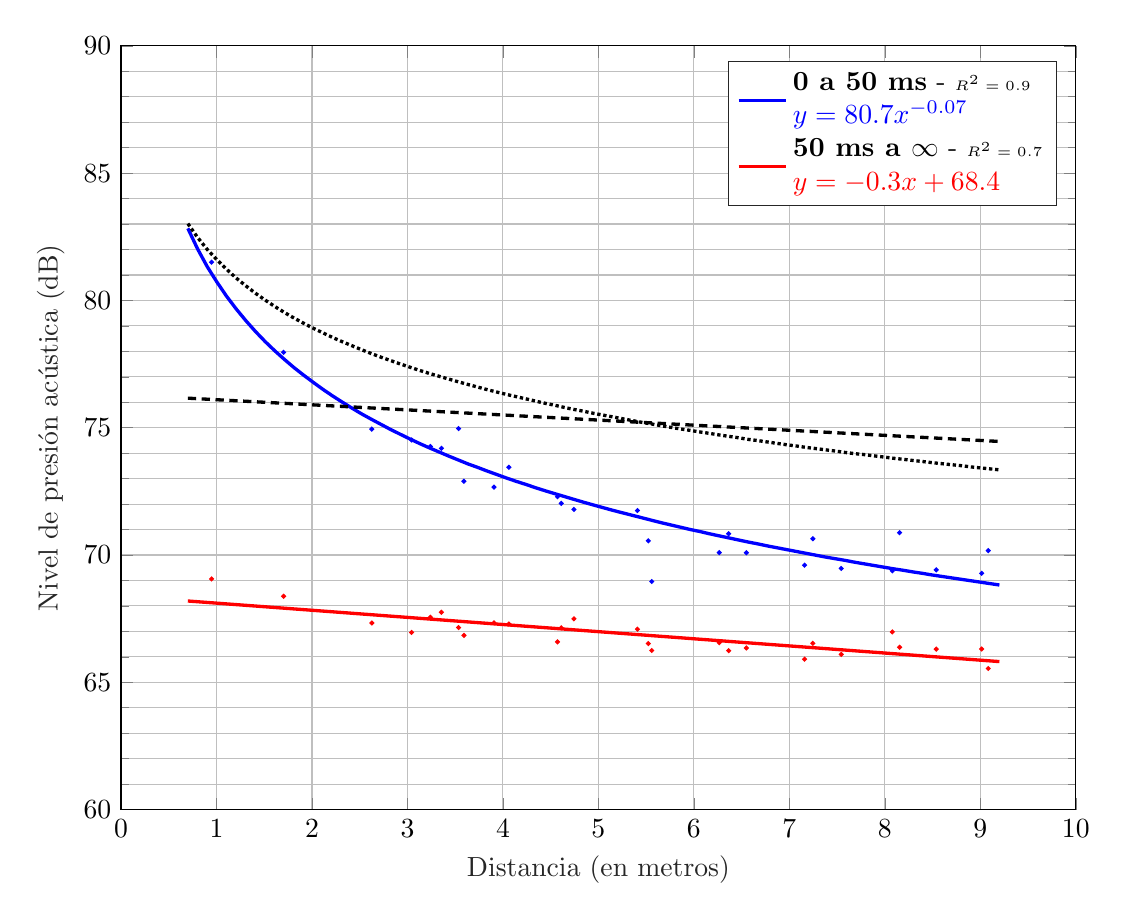
\begin{tikzpicture}

\begin{axis}[%
width=\textwidth,
height=0.8\textwidth,
at={(0\textwidth,0\textwidth)},
scale only axis,
xmin=0,
xmax=10,
xlabel style={font=\color{white!15!black}},
xlabel={Distancia (en metros)},
ymin=60,
ymax=90,
ylabel style={font=\color{white!15!black}},
ylabel={Nivel de presión acústica (dB)},
axis background/.style={fill=white},
xmajorgrids,
xminorgrids,
ymajorgrids,
yminorgrids,
minor y tick num= 4,
legend style={legend cell align=left, align=left, draw=white!15!black}
]
% Curvas CATT
\addplot[color=blue,domain=0.7:9.2, samples=85,line width=1.2]{80.73*x^(-0.072)};
\addlegendentry{\textbf{0 a 50 ms} - \tiny{$R^2 = 0.9$}\\$\color{blue}y = 80.7·x^{-0.07}$}

\addplot[color=red,domain=0.7:9.2, samples=85,line width=1.2]{-0.28*x+68.39};
\addlegendentry{\textbf{50 ms a $\infty$} - \tiny{$R^2 = 0.7$}\\$\color{red}y = -0.3·x+68.4$}

% Curvas in situ
\addplot[color=black,densely dotted,line width=1.2pt,domain=0.7:9.2, samples=85]{78.7*x^(-0.05)+2.9};
\addplot[color=black,densely dashed,line width=1.2pt,domain=0.7:9.2, samples=85]{-0.2*x+73.40+2.9};

% Puntos
\addplot [color=blue, only marks,mark size=0.7pt]
  table[row sep=crcr]{%
  0.948683298050514	81.5034022462516\\
1.70293863659264	77.9604720495982\\
2.62678510731274	74.9450056206266\\
3.04302481094059	74.5164853119413\\
3.24037034920393	74.2620379082671\\
3.35559234711250	74.1888946213408\\
3.53553390593274	74.9657493376305\\
3.59165699921359	72.8967181276975\\
3.90640499692492	72.6674994614721\\
4.06201920231798	73.4447542538069\\
4.57165178026498	72.2893786447318\\
4.61085675335940	72.0269191607698\\
4.74341649025257	71.7920610855486\\
5.40925133451941	71.7470474133201\\
5.52268050859363	70.5575249312815\\
5.55877684387492	68.9590671078746\\
6.26578007912822	70.0965854954904\\
6.36396103067893	70.8361666485416\\
6.54980915752513	70.0912217996624\\
7.15960892786750	69.6020991584691\\
7.24568837309472	70.6388641001404\\
7.54320886625844	69.4711599008487\\
8.07836617144828	69.3786993792196\\
8.15475321515005	70.8779927992126\\
8.53814968245463	69.4178255738047\\
9.01443287178955	69.2818532843703\\
9.08295106229248	70.1712672420559\\
  };
  
  \addplot [color=red, only marks,mark size=0.7pt]
  table[row sep=crcr]{%
  0.948683298050514	69.0614022592804\\
1.70293863659264	68.3789306872370\\
2.62678510731274	67.3305757179527\\
3.04302481094059	66.9599563309559\\
3.24037034920393	67.5537179622664\\
3.35559234711250	67.7505225752068\\
3.53553390593274	67.1500247730451\\
3.59165699921359	66.8427309755973\\
3.90640499692492	67.3393968502688\\
4.06201920231798	67.2906360577647\\
4.57165178026498	66.5896277965778\\
4.61085675335940	67.1423946944337\\
4.74341649025257	67.4933509242810\\
5.40925133451941	67.0859873464819\\
5.52268050859363	66.5216181182482\\
5.55877684387492	66.2501919867704\\
6.26578007912822	66.5596497676022\\
6.36396103067893	66.2436355563401\\
6.54980915752513	66.3492883390880\\
7.15960892786750	65.9096755815499\\
7.24568837309472	66.5306785734246\\
7.54320886625844	66.0974333054611\\
8.07836617144828	66.9797629598969\\
8.15475321515005	66.3778728334517\\
8.53814968245463	66.3054831839590\\
9.01443287178955	66.3088472266783\\
9.08295106229248	65.5428242170173\\
  };
\end{axis}
\end{tikzpicture}%